\subsection{Hysteresekurve}\label{sec:Aufgabe2}
teresekurve des Vollkerns durch graphische Auswertung der Messdaten.} \label{fig:Hysteresekurve}

\begin{figure}[H]
    \centering
    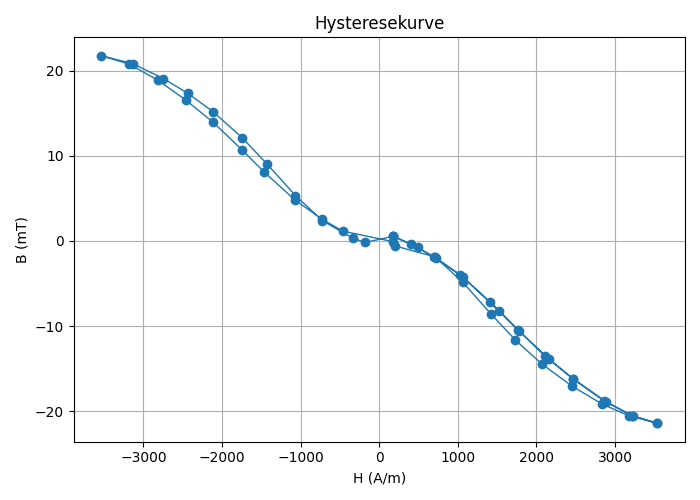
\includegraphics[width=0.4\linewidth]{Hysteresekurve-geschichteter Kern.png}
    \caption{Hysteresekurve des geblätterten Kerns durch graphische Auswertung der Messdaten.} \label{fig:HysteresekurveGeblaettert}
\end{figure}

\begin{figure}[H]
    \centering
    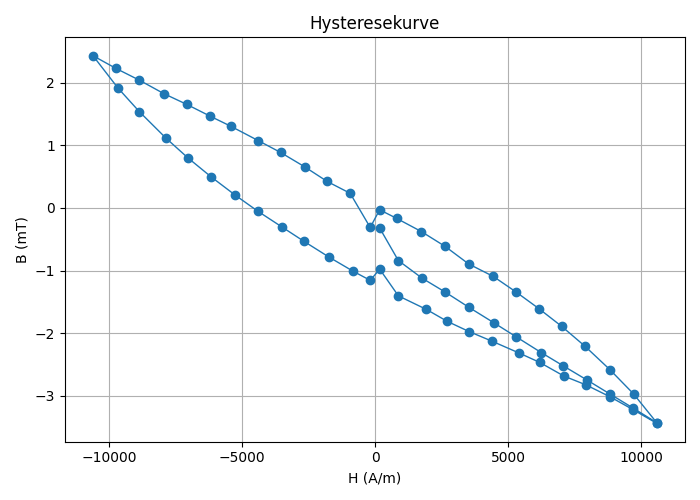
\includegraphics[width=0.4\linewidth]{Hysteresekurve-Vollkern.png}
    \caption{Hysteresekurve des Vollkerns durch graphische Auswertung der Messdaten.} \label{fig:HysteresekurveVollkern}
\end{figure}